\section{証明}
\label{section:differentiable}

本節では次の手順で定理\ref{DifferentiableIsPspace}, \ref{KTimesIsCH}を示す. 
まずある種の差分方程式の族が, 
$\classPSPACE$困難ないし$\classCH$困難であることを示す
(\ref{section:divp}節, \ref{subsection: counting hierarchy}節).
そしてこの差分方程式が, 
滑らかさの条件を満たす\eqref{eq:ode}の形の微分方程式の族により模倣されることを示す
(\ref{subsection: ode family}節). 
この族を一つの滑らかな微分方程式へ埋め込むことで, 
定理にいう$g$, $h$を構成する(\ref{subsection: proof of theorems}節).

このように微分方程式で差分方程式を模倣する考え方は, 
Lipschitz条件の場合の証明
\cite{kawamura2010lipschitz}にも本質的には既に現れていたものであるが, 
本稿ではより精密に, 滑らかさの条件が与える影響を調べるため, 
差分方程式をある種の回路族として定義する. 
その結果, 
$2$回以上連続微分可能という制限の下でも, 
回路の深さが小さければ模倣できることが判り, 
そのことから$\classCH$困難性が従う. 

\subsection{差分方程式}
\label{section:divp}

この節では微分方程式\eqref{eq:ode}の離散版ともいうべき差分方程式を
ある種の一様な回路族として定義し, 
それが深さの制限に応じて
$\classPSPACE$困難ないし$\classCH$困難であることを示す.

$[n] = \{0, \dots , n-1\}$と書く.
関数$G \colon [P] \times [Q] \times [R] \to \{-1, 0, 1\}$と
$H \colon [P + 1] \times [Q+1] \to [R]$が
任意の$i \in [P]$, $T \in [Q]$について以下を満たすとき(図\ref{fig:divp}), 
\begin{figure}
 \begin{center}
  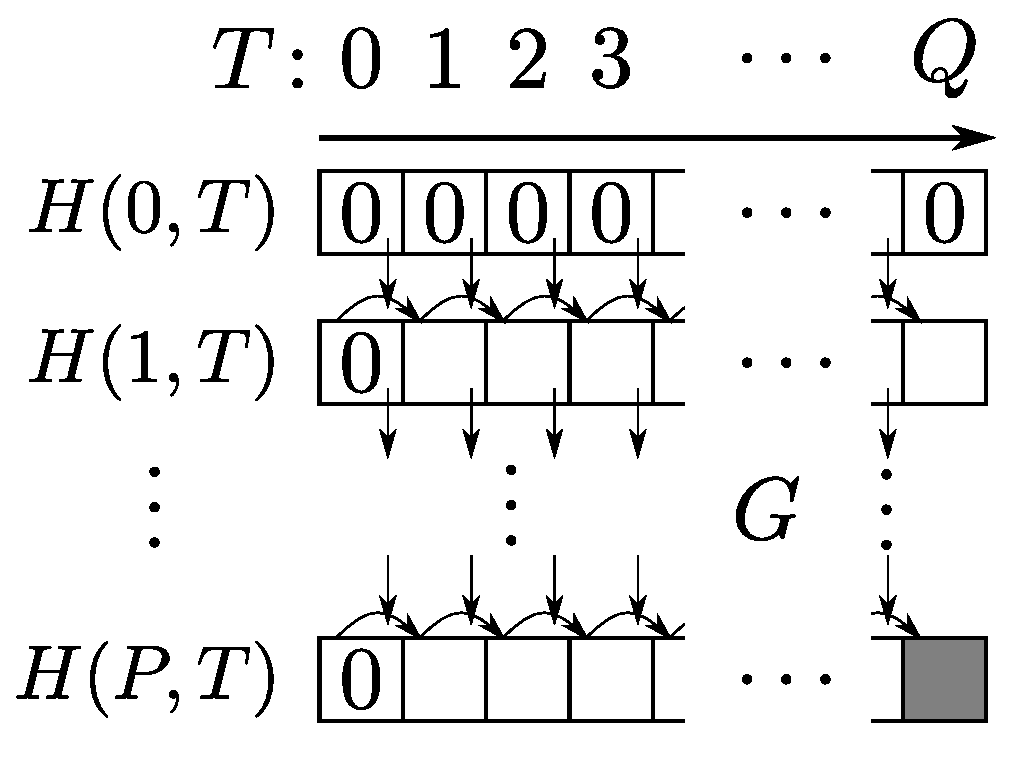
\includegraphics[height=0.15\textheight]{image/divp.eps}
 \end{center}
 \caption{差分方程式$G$とその解$H$}
 \label{fig:divp}
\end{figure}
$H$を\emph{差分方程式}\kern\xkanjiskip$G$の解と呼ぶ.
\begin{gather}
   H(i, 0) = H(0, T) = 0 \label{eq:initial value}
\\
   H(i + 1, T + 1) - H(i+1, T) = G(i, T, H(i, T))  \label{eq:divp}
\end{gather}
$P$, $Q$, $R$をそれぞれこの差分方程式の
\emph{段数}, \emph{列数}, \emph{欄の大きさ}と呼ぶ.
\eqref{eq:ode}の初期条件$h(0) = 0$と方程式$\D h(t) = g(t, h(t))$が
それぞれ式\eqref{eq:initial value}, \eqref{eq:divp}に似ており, 
\ref{subsection: ode family}節ではこれを用いて
微分方程式で差分方程式を模倣する. 

文字列$u$ごとに一つの差分方程式$G _u$を与え,
$u$が言語$L$に属するかをその差分方程式によって計算することを考える.
各 $u$ に対して $G_u$ の段数と列数, 解をそれぞれ $P_u, Q_u, H_u$ としたとき,
言語$L$が関数族$(G_u)_u$によって
\emph{認識}されるとは,
$H_u(P_u, Q_u) = L(u)$ を満たすこととする.

% このままでは任意の言語を差分方程式で認識可能となってしまうので, $(G_u)_u$全体にある種の制限をかける.
族$(G_u)_u$が\emph{一様}であるとは,
$G_u$の段数, 列数, 欄の大きさそれぞれを$u$を入力とする関数と見做したとき
それらが多項式時間計算可能であり,
かつ与えられた$(u, i, T, Y)$から$u$の多項式時間で$G_u(i, T, Y)$が
計算できることと定義する.
そのようなとき$G _u$の段数, 列数及び欄の大きさは,
$|u|$の多項式の指数($2^{\mathrm{poly} (|u|)}$)で抑えられる.
$G_u$ の段数がさらに $|u|$ の多項式, または対数のオーダーで抑えられるとき, 
族 $(G_u) _u$ はそれぞれ\emph{多項式段}, \emph{対数段}であるという. 
この用語を使うと, 
河村がLipschitz連続な場合の解析に用いた補題
\cite[補題4.7]{kawamura2010lipschitz}は次のように書ける. 

\begin{lemma}
 \label{DIVPpolyIsPSPACEhard}
 多項式段の一様な差分方程式族によって認識される$\classPSPACE$困難な言語が存在する
 \footnote{差分方程式によって認識される言語のクラスはカープ帰着において閉じており,
多項式段一様な関数族によって認識される言語は$\classPSPACE$と一致する.}.
\end{lemma}

河村\cite{kawamura2010lipschitz}は
この多項式段の一様な差分方程式族をLipschitz連続な微分方程式で模倣することで, 
表\ref{table:related}第三行の結果を得た. 
本稿の定理\ref{DifferentiableIsPspace}はこの構成に手を加えて, 
$(\infty, 1)$回微分可能な模倣に
作り替えることにより
(\ref{subsection: ode family}, \ref{subsection: proof of theorems}節), 
やはり補題\ref{DIVPpolyIsPSPACEhard}から得られる. 

本稿では更に, 対象とする差分方程式族を対数段に制限すれば, 
$(\infty, 2)$回以上微分可能な関数によっても
模倣できることを示し
(\ref{subsection: ode family}, \ref{subsection: proof of theorems}節), 
これと次の補題から定理\ref{KTimesIsCH}を得る. 

\begin{lemma}
 \label{DIVPlogIsCHhard}
 対数段の一様な差分方程式族によって認識される$\classCH$困難な言語が存在する.
\end{lemma}

計数階層$\classCH$の定義及び補題\ref{DIVPlogIsCHhard}の証明は
\ref{subsection: counting hierarchy}節にて行う.

\subsection{計数階層と対数段の差分方程式}
\label{subsection: counting hierarchy}

\emph{計数階層}\kern\xkanjiskip(Counting Hierarchy) $\classCH$は
Wagnerによって導入された計算量クラスである\cite{wagner1986complexity}.
多項式階層$\classPH$が$\classNP$の神託機械を用いて
\begin{align*}
 \classSigma^p_0  &= \classP
 &
 \classSigma^p_{n+1} &= \classNP ^{\classSigma^p_n}
 &
 \classPH &= \bigcup_n \classSigma^p_n
\end{align*}
と定義されるのに対し,
計数階層は多項式階層の$\classNP$を$\classPP$で置き換えて
\begin{align*}
 \quantC_0 \classP  &= \classP
 &
 \quantC_{n+1} \classP &= \classPP^{\quantC_n \classP}
 &
 \classCH &= \bigcup_n \quantC_n \classP
\end{align*}
で定義される\footnote{ただしこの特徴づけは Tor{\'a}n によるものであり,
Wagnerによる定義とは異なる\cite{toran1991complexity}.
}. $\classPH \subseteq \classCH \subseteq \classPSPACE$だが,
いずれも真の包含か否かは未解決である.

各階層$\quantC_n \classP$は次の完全問題$\quantC_n B_{be}$をもつ.
% $n$回の量化子交替を持つ命題論理式の評価は,
% 多項式階層の各階層$\classSigma^p_n$の完全問題であるが,
% 新たに計数用の量化子を導入して同様の判定問題を構成する.
量化子 $\quantC$ を自然数 $m$, $l$ 個の論理変数の組 $X$,
論理式$\phi(X)$について次のように定義する.
\begin{equation}
 \quantC^m X \phi(X) 
  \longleftrightarrow 
  \bigl|\{X \in \{0, 1\}^l \mid \phi(X) = 1\}\bigr| \ge m.
\end{equation}
$\quantC^1 = \exists$, $\quantC^{2^l} = \forall$ であり, $\quantC$ は $\exists, \forall$ の
一般化と言える.
言語$\quantC_n B_{be}$を次のように定義する.
\begin{equation}
 \langle \phi(X_1, \dots, X_n), m_1, \dots, m_n \rangle \in \quantC_n B_{be}
 \longleftrightarrow
 \quantC^{m_1}{X_1} \cdots \quantC^{m_n}{X_n} \phi(X_1, \dots, X_n) 
\end{equation}
ただし
$X_i$ は論理変数の組,
$\phi(X_1, \dots, X_n)$は$X_1, \dots, X_n$以外の変数を持たない論理式とする.

\begin{lemma}[{\cite[定理7]{wagner1986complexity}}] \label{lemma:CnP-complete}
 $\quantC_n B_{be}$ は $\quantC_n\classP$ 完全.
\end{lemma}

これらの問題$\quantC_n B_{be}$から問題$\quantC_{\log} B_{be}$を次で定義する.
\begin{equation}
 \langle 0^{2^n}, u \rangle \in \quantC_{\log} B_{be}
 \longleftrightarrow
 u \in \quantC_n B_{be}
\end{equation}
% 入力として階層の指数サイズ($0^{2^n}$)を与えているのは, padding することにより
% 量化子の数が全体の入力長に対して対数オーダーであることを保証することで,
% 対数段の差分方程式により認識可能とするためである.
この$\quantC_{\log} B_{be}$が補題\ref{DIVPlogIsCHhard}で求める言語であること,
つまり$\classCH$困難かつ対数段一様関数族によって認識可能であることを示す.

\begin{proof}[\textup{補題\ref{DIVPlogIsCHhard}の証明}]
 $\quantC_{\log} B_{be}$が$\classCH$困難であることを示す.
 任意の $\classCH$ の言語 $A$ はある階層 $\quantC_n \classP$ に属する. 
 補題 \ref{lemma:CnP-complete} より任意の $u \in \{0,1\}^*$ について
 $u \in A \leftrightarrow f(u) \in \quantC_n B_{be}$ 
 を満たす多項式時間関数 $f$ が存在する.
 \begin{align}
  u \in A 
  & \longleftrightarrow \langle 0^{2^n}, f(u) \rangle \in \quantC_{\log} B_{be}
 \end{align}
 $n$ は定数であるため $\langle 0^{2^n}, f(\cdot) \rangle$ は多項式時間関数.
 よって $A$ は $\quantC_{\log} B_{be}$ に帰着する.


 $\quantC_{\log} B_{be}$を認識する関数族 $(G_u)_u$, 
 その解$(H_u)_u$, 関数 $p \colon \N \to \N$, 多項式 $q,r$ を構成する.
 自然数 $n, m_1, \dots, m_n$, 論理式$\phi$を
 $u  = \langle 0^{2^n}, 
 \langle \phi(X_1, \dots, X_n), m_1, \dots, m_n \rangle \rangle$
 を満たすものとする. 
 (そのような$n, m_1, \dots, m_n, \phi$が存在しないとき$u \not \in A$.)
 
 
 $L = \quantC_{\log} B_{be}$, $l_i = |X_i|$と表記する.
 関数 $C^m \colon \N \to \N$ を
 \begin{equation}
  C^m(x) 
     = \begin{cases}
       1 & (x \ge m) \\
       0 & (x < m) \end{cases}
 \end{equation}
 と定義する. 
 任意の $i = 0, \dots, n$ と $n-i$ 個の文字列 
 $Y_{i+1} \in \{0,1\}^{l_{i+1}}, \dots, Y_n \in \{0,1\}^{l_n}$ 
 について論理式
 $\quantC^{m_{i}}{X_i} \cdots \quantC^{m_1}{X_1}
 \phi(X_1, \dots, X_i, Y_{i+1}, \dots, Y_n)$
 の真偽値を $\phi_i(Y_{i+1}, \dots, Y_n)$ と表記する.
 \begin{align}
  \phi_0 (Y_1, \dots, Y_n) &= \phi(Y_1, \dots, Y_n)
  \\ \label{eq:phi-step}
  \phi_{i+1}(Y_{i+2}, \dots, Y_n) 
  &= C^{m_{i+1}}\left(\sum\nolimits_{X_{i+1} \in \{0,1\}^{l_i}} 
  \phi_i(X_{i+1}, Y_{i+2}, \dots, Y_{n})\right) 
  \\
  \phi_n() &= L(u) 
 \end{align}
 $T \in \N$ に対し, $T_i$ を $T$ の2進表記における $i$ 桁目, 
 $T_{[i,j]} = T_{j-1} T_{j-2} \cdots T_{i+1} T_{i}$ と表記する.


 $s_i = i + \sum^i_{j=1}l_j$ と書く.
 $G_u$ を $(i, T, Y) \in [n+1] \times [2^{s_n}+1] \times [2^{|u|}]$ の範囲で
 を以下のように定義する. 一段目つまり $i=0$ ならば
 \begin{equation}
  G_u(0,T,Y) = 
   (-1)^{T_{s_1}}\phi(T_{[1,s_1]}, T_{[s_1+1,s_2]},
    \dots, T_{[s_{n-1}+1,s_n]}) 
 \end{equation}
 $i \ge 1$ ならば
 \begin{equation} \label{eq:def-Gu:case0}
  G_u(i,T,Y) = 
   \begin{cases}
    (-1)^{T_{s_{i+1}}} C^{m_i}(Y) 
    & (T_{[1,s_i]} = 10 \cdots 0) \\
    0 & (\text{othewise}).
   \end{cases} 
 \end{equation}


 任意の $i \in [n+1]$, $T \in [2^{s_n}+1]$ について,
 $H_u(i,T) \in [2^{l_i}+1]$ が成りたつこと,
 および $T_{[1,s_i]} = 10 \cdots 0$ ならば
 \begin{equation} \label{eq:subformula}
  G_u(i,T,H_u(i,T)) = (-1)^{T_{s_{i+1}}} 
   \phi_i(T_{[s_i+1, s_{i+1}]}, \dots, T_{[s_{n-1}+1, s_n]})
 \end{equation}
 を満たすことを $i$ についての帰納法により示す.
 上記が成り立つとき,
 $i=n$, $T=2^{s_n}$ において $G_u(n, 2^{s_n}, H_u(n,2^{s_n})) = \phi_n() = L(u)$
 よって $H_u(n+1, 2^{s_n}+1) = L(u)$.
 ここで 
 \begin{gather}
  n+1 \le \log(|0^{2^n}|) + 1 = O(\log(|u|)) \\
  2^{s_n}+1 \le 2^{s_n+1} \le 2^{|u|}
 \end{gather}
 より $l(u) = n+1, q(x) = r(x) = x$ とおき $G_u$ を
 $[l(u)] \times [2^{q(|u|)}] \times [2^{r(|u|)}]$ の範囲に拡張すると
 $H_u(p(u), 2^{q(|u|)}) = L(u)$.

 $i=0$ のとき, 式(\ref{eq:def-Gu:case0})より成り立つ.
 $i=j$ のとき, 成り立つと仮定する, $Y = H_u(i+1, T)$ とおくと
 \begin{align}
  Y 
  &= \sum_{V = 1}^{T-1} G_u(i, V, H_u(i, V)) \\
  &= \sum (-1)^{V_{s_{i+1}}} \phi_i(V_{[s_i+1, s_{i+1}]}, 
   \dots, V_{[s_{n-1}+1, s_n]})
 \end{align}
 $T_{[1, s_{i+1}]} = 10 \cdots 0$ のとき,
 $V_{[1, s_n]} = T_{[s_{i+1}+1,s_n]} 0 X 1 0 \cdots 0$ であるとき
 以外の値は打ち消し合うので,
 \begin{equation}
  Y = \sum\nolimits_{X \in \{0,1\}^{l_i}} 
  \phi_i(X, T_{[s_{i+1}+1, s_{i+2}]}, \dots, T_{[s_{n-1}+1, s_n]})
 \end{equation}
 式(\ref{eq:phi-step})より
 \begin{align}
  G_u(i+1,T,H_u(i+1,T)) 
  &= (-1)^{T_{s_{i+2}}} C^{m_{i+1}} (Y)\\
  &= (-1)^{T_{s_{i+2}}} \phi_{i+1}(T_{[s_{i+1}+1, s_{i+2}]}, \dots, T_{[s_{n-1}+1, s_n]})
 \end{align}
 よって $i=j+1$ でも成り立つ.
 \end{proof}



\subsection{差分方程式を模倣する関数族}
\label{subsection: ode family}
次に前節で示した$\classPSPACE$または$\classCH$困難な各差分方程式を滑らかな実関数で模倣可能であることを示す.

しかし補題を述べる前に実関数の多項式時間計算可能性を
実関数族のそれに拡張する.
文字列$u$で添字づけられた実関数$f _u \colon A \to \R$の
族 $(f_u)_u$ を機械 $M$ が計算するとは,
任意の実数 $x \in A$, 任意の $x$ の名 $\phi_x$ に対して,
文字列 $v$ を $M ^{\phi _x} (u, v)$ へ移す関数が, 
$f _u (x)$ の名であることをいう.
実関数族が多項式時間計算可能であるとは, その実関数族を計算する
多項式時間神託機械が存在することである.

 \begin{lemma}
  \label{KTimesFamily}
  或る $\classCH$ 困難な言語 $L$,
  二変数多項式 $\mu$ において,
  任意の正の整数 $k$,
  任意の多項式 $\gamma$ に対して,
  多項式 $\rho$, 実関数族 $(g_u)_u, (h_u)_u$ で, 
  $(g_u)_u$ は多項式時間計算可能であり,
  各文字列 $u$ に対して以下を満たすものが存在する.

  \begin{enumerate}
   \item \label{enum:kf:start}
     $g_u\colon [0,1] \times [-1,1]\to \R, \quad h_u\colon [0,1] \to [-1,1]$; 
   \item $g_u$と$h_u$は常微分方程式 (\ref{eq:ode}) を満たす;
   \item $g_u$ は $(\infty, k)$ 階連続微分可能;
   \item \label{enum:boundary}
	 任意の $i \in \N$, $y \in [-1,1]$ に対して
	 \begin{equation*}
	  \D^{(i, 0)} g_u(0,y) = \D^{(i, 0)} g_u(1,y) = 0 ;
	 \end{equation*}
   \item \label{enum:smooth}
	 任意の $i \in \N$, $j \in \{0, \dots, k\}$ に対して
	 \begin{equation*}
	  \left|\D^{(i,j)} g_u(t,y)\right| \le 2^{\mu(i, |u|) - \gamma(|u|)};
	 \end{equation*}
   \item \label{enum:kf:end}
	 $h_u(1) = 2^{-\rho(|u|)} L(u)$.
  \end{enumerate}
 \end{lemma}

\begin{lemma}
 \label{DifferentiableFamily}
 或る $\classPSPACE$ 困難な言語 $L$,
 二変数多項式 $\mu$ において,
 $k = 1$のとき,
 任意の多項式 $\gamma$ に対して,
 多項式 $\rho$, 実関数族 $(g_u)_u, (h_u)_u$ で, 
 $(g_u)_u$ は多項式時間計算可能であり,
 各文字列 $u$ に対して
 補題\ref{KTimesFamily}の(\ref{enum:kf:start}) -- (\ref{enum:kf:end})を満たすものが存在する.
\end{lemma}



 この補題より各 $h_u(1)$ に $L(u)$ の情報を持つ
 滑らかな実関数族 $(g_u)_u, (h_u)_u$ の存在が示される.
 河村によるLipschitz連続な常微分方程式の$\classPSPACE$困難性の証明における,
 補題4.1 に対応するが,
 $g$ を微分可能にするため, 条件 (iii) -- (v) が付け加えられている.


 この補題の証明の基本的な流れを説明する.
 ある$\classCH$困難(resp. $\classPSPACE$困難)な言語$L$に対し, 
 補題 \ref{DIVPlogIsCHhard}(resp. 補題 \ref{DIVPpolyIsPSPACEhard})
 を用いて $L$ を認識する $(G_u)_u$ 
 及び $(H_u)_u$ を得る.
 そして各 $G_u, H_u$ を模倣する
 滑らかな $g_u \colon [0,1] \times [-1, 1] \to \R$ 
 と $h_u \colon [0,1] \to \R$ 構成する.
 それらが常微分方程式(\ref{eq:ode})を満たすことを差分方程式の性質により示し,
 $(g_u)_u$の多項式時間計算可能性を$(G_u)_u$ の一様性から示す.

 上記の証明は基本的に, 河村による証明と変わらない\cite[補題4.1]{kawamura2010lipschitz}.
 河村の証明と大きく異なる点は, $g_u$ を滑らかな関数にするため, 
 以下のような無限回微分可能な多項式時間実関数 $f \colon [0,1] \to \R$ を用いて
 $g_u$ を構成していることである.

 \begin{lemma}[{\cite[補題 3.6]{ko1991complexity}}]
  \label{SmoothFunction}
  以下を満たす多項式時間計算可能で無限回微分可能な
  実関数 $f \colon [0,1] \to \R$ が存在する.

  \begin{enumerate}
   \item $f(0) = 0, \quad f(1) = 1$;
   \item 任意の $n \ge 1$ で $f^{(n)}(0) = f^{(n)}(1) = 0$;
   \item $f$ は $[0,1]$ で単調増加;
   \item 任意の $n \ge 1$ で $\D^n f$ は多項式時間実関数.
  \end{enumerate}
 \end{lemma}

 さらにここでは上記の条件に加えて, 
 \begin{enumerate}
  \setcounter{enumi}{4} 
  \item 以下を満たす多項式$s$が存在する
	\begin{equation} \label{enum:polynomial-size}
	 |\D^n f| \le s(n)
	\end{equation}
 \end{enumerate}
 を満たすような$f$が存在することを用いて証明する.
 葛による証明を確認することで多項式$s$の存在は容易に示される.

 ここではより難しく一般的な補題 \ref{KTimesFamily} のみ証明を行い,
 補題 \ref{DifferentiableFamily} について証明は省略する.


 \begin{proof}[\rm 補題 \ref{KTimesFamily} の証明]
  補題 \ref{DIVPlogIsCHhard} より
  $\classCH$ 困難な言語 $L$ を認識する
  対数段一様関数族 $(G_u)_u$, その解 $(H_u)_u$を得る.
  対数段一様関数族の定義より 
  $G_u \colon [l(|u|)] \times [2^{q(|u|)}] \times [2^{r(|u|)}] \to \{-1, 0, 1\}$
  を満たす関数$l$, 多項式 $q,r$が存在する. 

  河村による証明と同様に$(G_u)_u, (H_u)_u$を拡張することにより,
  以下のことを仮定する.
  \begin{gather}
   H_u(i, 2^{q(|u|)}) = \begin{cases}
			L(u) & (i=p(|u|)) \\
			0 & (i<p(|u|)).
			\end{cases}
   \\
   i \not = j_u(T)  \to G_u(i, T, Y) = 0 
  \end{gather}
  
  $H_u$を模倣するような$h_u$を構成する.
  具体的には$h_u(T/2^{q(|u|)}) = \sum^{l(|u|)}_{i}H_u(i, T)/B^{d_u(i)}$
  を満たすように$h_u$を構成する. ここで$d_u$は段数から桁への割り当てである.
  $l(x) = O(\log x)$より任意の$x \in \N$に対して,
  $(k+1)^{l(x)} \le p(x)$を満たす多項式$p$が存在する.
  $B$と関数$d_u \colon [l(|u|)+1] \to \N$を
  \begin{align*}
   B &= 2^{\gamma(|u|) + r(|u|) + s(k) + k + 3}
   &
   d_u(i) &= 
   \begin{cases}
    p(|u|) & (i=l(|u|)) 
    \\
    (k+1)^i & (i<l(|u|))
   \end{cases}
  \end{align*}
  とおく.
 各 $(t, y) \in [0,1] \times [-1, 1]$ に対して,
 $t = (T + \theta)2^{-q(|u|)}$, $y = (Y + \eta)B^{-d_u(j_u(T))}$ を満たす
 自然数 $N$, $\theta \in [0,1)$, 整数 $Y$, $\eta \in [-1/4, 3/4)$ 
 がそれぞれ唯一存在する.
 関数$\delta_{u,Y} \colon [0,1] \to \R$を
 \begin{equation} \label{eq:delta}
  \delta_{u, Y} (t) = \frac{2^{q(|u|)} \D f(\theta)}{B^{d_u(j_u(T)+1)}} 
   G_u\left( j_u(T),\ T,\ Y \bmod 2^{r(|u|)} \right)
 \end{equation}
 とおき, $g_u, h_u$ を以下のように定義する.
 \begin{equation}
  \label{eq:gu}
\\  g_u(t,y) 
  = \begin{cases}
     \delta_{u, Y}(\theta)
     & (\eta \le \frac 1 4)
     \\
     ( 1-f ( \frac{4\eta-1}{2})) \delta_{u, Y}(\theta) 
     + f ( \frac{4\eta-1}{2}) \delta_{u,Y+1}(\theta)
     & (\eta > \frac 1 4)
    \end{cases}
 \end{equation}
 \begin{equation} 
  h_u(t) 
   = \sum^{l(|u|)}_{i=0} \frac{H_u(i, T)}{B^{d_u(i)}}  
  + \frac{f(\theta)}{B^{d_u(j_u(T)+1)}} G_u(j_u(T), T, H_u(j_u(T), T)) 
  \label{eq:hu}
 \end{equation}
  ただし$f$と多項式$s$は補題 \ref{SmoothFunction}
  および式(\ref{enum:polynomial-size})を満たすものとする.


 上記のように定義した $g_u, h_u$ が補題\ref{DifferentiableFamily} で求める
 性質を満たすことを示す. ただし多くは河村による証明と同様に示せるため
  異なる条件 (iii) - (vi) のみ示す
 
  $g_u$ が $(\infty, k)$ 階連続的微分可能であることを示す.
  $\eta$ が $[-1/4, 1/4]$ と $[1/4, 3/4]$ である区間それぞれにおいて微分する.
  任意の $i \in \N$ について

  \begin{equation}
   \D^i \delta_{u,Y}(t) 
    = \frac{2^{(i+1)q(|u|)} \D^{i+1}f(\theta)}{B^{d_u(j_u(T)+1)}}
    G_u\left( j_u(T),\ T,\ Y \bmod 2^{r(|u|)} \right)
  \end{equation}

  \begin{equation}
   \label{eq:derivativeofgu}
    \D^{(i,0)} g_u(t, y)
     = \begin{cases}
 	\D^i \delta_{u, Y}(\theta) 
	\hfill (- \frac 1 4 < \eta < \frac 1 4) \\
	\left( 1-f \left(\frac{4\eta-1}{2}\right)\right) 
	\D^i \delta_{u, Y}(\theta) 
	+ f \left(\frac{4\eta-1}{2}\right) \D^i \delta_{u,Y+1}(\theta) \\
	\hfill (\frac 1 4 < \eta < \frac 3 4)
       \end{cases}
  \end{equation}   
  $j \in \{1, \dots , k\}$ について,

  \begin{equation}
    \D^{(i,j)} g_u(t, y)
     = \begin{cases}
	0 \hfill (- \frac 1 4 < \eta < \frac 1 4) \\
	(2B^{d_u(j_u(T))})^j \D^j f(\frac{4\eta - 1}2)
	(\D^i \delta_{u,Y+1}(\theta)-\D^i \delta_{u, Y}(\theta)) \\
	\hfill (\frac 1 4 < \eta < \frac 3 4)
       \end{cases}
  \end{equation}
  境界においても連続であるため,
  $g_u$ は $(\infty, j)$ 階連続的微分可能であることが示された.
  式 (\ref{eq:derivativeofgu}) に $t = 0, 1$ ($\theta = 0$) を代入して
  $\D^{(i, 0)} g_u(0,y) = \D^{(i, 0)} g_u(1,y) = 0$.

  (\ref{enum:smooth})を示す.
  $\mu(x, y) = (x+1)q(y) + s(x+1)$とおく(この$\mu$は$k$や$\gamma$に依存しない).
  式(\ref{eq:delta})より
  $|\D^i \delta_{u,Y}(t)| \le 2^{(i+1)q(|u|) + s(i+1)}B^{-d_u(j_u(|u|)+1)}$.
  任意の $i \in \N$, $j \in \{0, \dots, k\}$ について
  \begin{equation}
   |\D^{(i,j)} g_u| 
   \le 
   2^k B^{k \cdot j_u(T)} 2^{s(k)} \cdot 2 \cdot 
   \frac{2^{(i+1)q(|u|) + s(i+1)}}{B^{d_u(j_u(|u|)+1)}} 
   \le
   \frac{2^{\mu(i, |u|) + s(k) + k + 1}}{B}
  \end{equation}
  $B$のとり方により, $|\D^{(i,j)} g_u| \leq 2^{\mu(i, |u|) - \gamma(|u|)}$.

  $\rho(x) = p(x) \cdot (\gamma(x)+r(x)+s(k)+k+3)$ とおくと,
  \begin{equation}
   h_u(1) = \frac{H_u(l(|u|), 2^{q(|u|)})}{B^{d_u(l(|u|))}} 
          = \frac{L(u)}{2^{p(|u|) \cdot (\gamma(|u|)+r(|u|)+s(k)+k+3)}}
	  = 2^{-\rho(|u|)} L(u).
  \end{equation}
 \end{proof}



 補題 \ref{DifferentiableFamily} の証明では
 $\classPSPACE$困難な言語を認識する多項式段一様関数族$(G_u)_u$とその解$(H_u)_u$に対して式(\ref{eq:delta}), (\ref{eq:gu}), (\ref{eq:hu})をそれぞれ,
 \begin{align}
  \delta_{u, Y} (t) &= \frac{2^{q(|u|)} \D f(\theta)}{B^{{j_u(T)+1}}} 
   G_u\left( j_u(T),\ T,\ Y \bmod 2^{r(|u|)} \right)
  \\
  g_u(t,y) 
  &= \begin{cases}
     \delta_{u, Y}(t)
     & (\eta \le \frac 1 4)
     \\
     ( 1-f ( \frac{4\eta-1}{2})) \delta_{u, Y}(t) 
     + f ( \frac{4\eta-1}{2}) \delta_{u,Y+1}(t)
     & (\eta > \frac 1 4)
    \end{cases}
  \\
  h_u(t) &= \sum^{l(|u|)}_{i=0} \frac{H_u(i, T)}{B^{i}}  
  + \frac{f(\theta)}{B^{{j_u(T)+1}}} G_u(j_u(T), T, H_u(j_u(T), T)) 
 \end{align}
 と置き換える. ただし$p, q, r$ は $G_u \colon [p(|u|)] \times [2^{q(|u|)}] \times [2^{r(|u|)}] \to \{-1, 0, 1\}$を満たす多項式.
 $(g_u)_u$と$(h_u)_u$が補題 \ref{DifferentiableFamily} で求める性質を満たすことは,
 補題 \ref{KTimesFamily} の証明と同様に示される.


\subsection{主定理の証明}
\label{subsection: proof of theorems}

 証明の概略を示す.
 前の節の補題から得られる $(g_u)_u$ と $(h_u)_u$ を縮小して連結し滑らかな $g$ と
 解 $h$ を構成する.
 $[0,1)$ を無限の区間に分割し, 各文字列 $u$ に対応する区間
 $[l^-_u, c_u]$ に $h_u$ を縮小して埋め込む. 
 ただし次の文字列 $u'$ の計算に影響を与えないために,
 $h_u$ を定義域方向について反転したものを
 区間 $[c_u, l^+_u]$ に埋め込むことで影響を相殺する.
 つまりある多項式$\rho'$に対して
 $h(l^-_u) = 0,\ h(c_u) = 2^{-\rho'(|u|)} L(u),\ h(l^+_u) = 0$ を満たす
 ように $h_u(t)$埋め込む.
 同様に $g$ は $h$ が常微分方程式の解となるよう,
 各文字列 $u$ に対応する区間に $g_u$ を縮小して埋め込む.

 定理 \ref{DifferentiableIsPspace} と定理 \ref{KTimesIsCH} の関係は
 補題 \ref{DifferentiableFamily} と補題 \ref{KTimesFamily} の関係と等しい.
 つまり $\classPSPACE$ が $\classCH$ に置き換わり,
 $(\infty, 1)$ 回連続微分可能が $(\infty, k)$回連続微分可能に一般化されている.
 よって定理 \ref{DifferentiableIsPspace} の証明は
 定理 \ref{KTimesIsCH} の証明から構成できるため省略する.

\begin{proof}[\rm 定理 \ref{KTimesIsCH} の証明]
 $L$ を $\classCH$ 困難な言語とおく.
 $L$ に対して補題 \ref{DifferentiableFamily} を用いて,
 まず多項式 $\mu$ をえる.
 \begin{align}
  \lambda(x) &= 2x + 2,&
  \gamma(x) &= x\mu(1, x) + x \lambda(x)
 \end{align}
 とおき, 各 $u$ に対して 
\begin{align}
 \Lambda_u 
 &= 2^{\lambda(|u|)}, &
 c_u 
 &= 1-\frac{1}{2^{|u|}}+\frac{2\bar{u}+1}{\Lambda_u}, &
 l_u^\mp 
 &= c_u\mp\frac{1}{\varLambda_u} 
\end{align}  
 とおく. ただし $\bar u \in \{0, \dots, 2^{|u|} - 1\}$ は $u$ を二進数と
 して解釈した数.
 $\gamma$ に対して, 補題より $\rho$, $(g_u)_u$, $(h_u)_u$ を得る.


 任意の $[0,1)$ の実数に対して,
 $l^\mp_u \pm \frac{t}{\Lambda_u}$ がその実数と等しくなるような
 $u, \pm, t\in [0,1]$ が存在する.
 関数 $g, h$ を $t \in [0,1)$, $y \in [-1, 1]$ に対して,
 \begin{align}
 g \left(l^\mp_u \pm \frac{t}{\Lambda_u}, \frac{y}{\Lambda_u}\right)
  &= \begin{cases}
      \pm \displaystyle \sum_{l=0}^k \frac{\D^{(0,l)}g_u(t,1)}{l!} (y-1)^l 
      &  (1<y) \\
      \pm g_u(t, y)      & (-1 \le y \le 1) \\
      \pm \displaystyle \sum_{l=0}^k \frac{\D^{(0,l)}g_u(t,-1)}{l!} (y+1)^l  
      &  (1<y) \\
    \end{cases} 
  \\
 h \left( l^\mp_u \pm \frac{t}{\Lambda_u} \right) 
  & = \frac{h_u(t)}{\Lambda_u}.
\end{align}
 $t=1$のとき $g(1,y) = 0$, $h(1) = 0$ と定義する.

 この $g$ が多項式時間計算可能であり $h$ が常微分方程式の解であることは,
 Lipschitz条件の場合と同様に示されるため,
 河村による証明を参照されたし\cite[定理3.2]{kawamura2010lipschitz}.
 ここでは特に$g$が$(\infty, k)$回連続微分可能であることのみ示す.

 $g_u$ は $(\infty, k)$ 階連続的微分可能であるため,
 各区間においては$(\infty, k)$ 階連続的微分可能である.
 $i \in \N$, $j \in \{0, \dots, k\}$, $t \in (0, 1)$ において
\begin{equation}
   \D^{(i, j)}g \left(l^\mp_u \pm \frac{t}{\Lambda_u}, \frac{y}{\Lambda_u}\right)
   = \begin{cases}
      \pm \Lambda_u^{(i, j)} \sum^{k}_{l=j} \frac{\D^{(i,l)} g_u(t,1)}{(l-j)!}
      (y - 1)^l &  (1<y)
      \\
      \pm \Lambda_u^{(i,j)} \D^{(i, j)} g_u(t, y) & (-1 < y < 1)
      \\
      \pm \Lambda_u^{(i, j)} \sum^{k}_{l=j} 
      \frac{\D^{(i,l)} g_u(t, -1)}{(l-j)!} (y + 1)^l &  (1<y)
    \end{cases}
\end{equation}
 $\D^{(i,j)}g_u$ は連続であるため 
 $t \in (0,1)$, $y \not = -1, 1$ において連続.
 境界($t = 0, 1$または$y = -1, 1$)において連続であることは,
 定義および補題 \ref{KTimesFamily} (\ref{enum:boundary})によりしめされる.
 第一変数が $1$ のとき連続であることを示す.
 補題 \ref{KTimesFamily} の(\ref{enum:smooth})より
 \begin{align*}
  \left|\D^{(i, j)}g \left(l^\mp_u \pm \frac{t}{\Lambda_u},
  \frac{y}{\Lambda_u}\right)\right|
  &\le 
  \Lambda_u^{i+j} \sum^{k}_{l=j} \left(|\D^{(i,l)} g_u |(\Lambda_u + 1)^l \right)
  \\
  & \le \Lambda_u^{i+j+k}  2^{k + \mu(i, |u|) - \gamma(|u|)}
  \\
  & =  2^{(i+j+k)\lambda(|u|) + k + \mu(i, |u|)  - \gamma(|u|)}.  \taghere
  \label{eq:sizeofderivative}
 \end{align*}
 $\gamma$ のとり方により, $|u| \to \infty$ のとき 
 式 (\ref{eq:sizeofderivative}) は 0 に収束する.
 よって  $\lim_{t \to 1-0}\D^{(i,j)} g(t,y) = g(1, y) = 0$.
 以上により $g$ は $(\infty, k)$ 階連続的微分可能.
\end{proof}


